\documentclass[]{book}

\usepackage[T1]{fontenc}
\usepackage[top=1in, bottom=1.5in, left=1in, right=1in]{geometry}

\usepackage[english]{babel}
\usepackage[autostyle]{csquotes}

\usepackage{upquote}

\usepackage{indentfirst}
\usepackage{float}

\usepackage{tikz}
\usepackage{tikz-uml}
\usetikzlibrary{shapes,arrows}

\usepackage{listings}

% Define block styles
\tikzstyle{block} = [rectangle, draw, fill=blue!20, 
text width=1.5in, minimum height=4em]
\tikzstyle{line} = [draw, -latex']

\usepackage{parskip}
\setlength{\parskip}{6pt}
\setlength{\parindent}{0pt}

\usepackage{hyperref}
\hypersetup{
	colorlinks,
	citecolor=black,
	filecolor=black,
	linkcolor=black,
	urlcolor=black
}


\renewcommand{\arraystretch}{1.25}

% Title Page
\title{Bonsai Project Technical Documentation}
\author{Andrew Benedict	<dev@andybenedict.com>}


\begin{document}
\maketitle
\tableofcontents

\chapter*{Introduction}

The Bonsai Project is an API for managing content, data structures, and their corresponding templates.

Aside from a small number of syntactic rules and interfaces required to facilitate it's basic operation, all Bonsai core components can be extended, overridden, or reconfigured to conform to the user's specific needs. The Bonsai development team strives to make as few assumptions as possible to maximize the control the user has over data structures, processors, and templates.

As a result of this control, the Bonsai project is not intended to be a content management system akin to the mainstream all-in-one solutions. Rather, it is intended to be used in custom development projects to provide an abstraction layer for managing templates and static content with built in support for mapping dynamic content into the generated output.

\section*{Features}

\begin{itemize}
	\item Simple tree structure
	\item Recursive creation and rendering
	\item Easy-to-customize templates
	\item Optional preprocessing of fields in templates
	\item Automated resolution of localized content
	\item Field mapping of dynamic content
	\item Dynamic fields have optional callback for conversion or formatting.
\end{itemize}

\chapter{Database}

The Bonsai Project uses a handful of database tables to store information, they can be divided into two groups:

\begin{itemize}
	\item Content
	\item Node
\end{itemize}

\section{Content Tables}

\subsection{Content Registry Table}

The primary table in the content part of the database is the content registry. 

\begin{figure}[H]
	\centering
	\caption{Content Registry Table}
	\vspace{12pt}
	\begin{tabular}{ |p{1.25in}|p{.75in}|p{2in}|p{1in}| }
		\hline
		\multicolumn{4}{|l|}{\textbf{contentRegistry}} \\
		\hline
		\hline
		Name & DataType & Keys & Notes\\
		\hline
		id & Int & PK & \\
		reference & Varchar & Unique & \\
		contentTypeID & Int & Foreign: contentType.id & \\
		dataFormat & Varchar & & \\
		contentCategoryID & Int & Foreign: contentCategory.id & \\
		startDate & Timestamp & & \\
		endDate & Timestamp & & \\
		active & Boolean & & \\
		\hline
	\end{tabular}
\end{figure}

Two fields are present for searching purposes, contentType being the primary and contentCategory being the secondary. For example, Bonsai natively has two contentTypes, BonsaiNode and Vocab. BonsaiNodes are complex datatypes intended to be paired with a template in the render tree. On the other hand, are plain text and useful for things like labels, or mapping the same term into multiple locations. See the \nameref{sec:vocabExamples} section of the \nameref{chapter:commonUsageExamples} chapter for further information.

There are two methods provided for limiting the display of content. 

The startDate and endDate fields allow scheduling of content either as part of the node tree or using dynamic nodes. (See the \nameref{sec:dynamicNode} in the \nameref{chapter:commonUsageExamples} chapter for further information.)

Setting active to false merely makes the content unavailable. This allows the data to be preserved for future use or alteration without making available to the content system.

\subsection{Content Table}

As the name implies, the content table stores the actual content associated with items listed in the contentRegistry.

\begin{figure}[H]
	\centering
	\caption{Content Table}
	\vspace{12pt}
	\begin{tabular}{ |p{1.25in}|p{.75in}|p{2in}|p{1in}| }
		\hline
		\multicolumn{4}{|l|}{\textbf{content}} \\
		\hline
		\hline
			Name & DataType & Keys & Notes\\
		\hline
			id & Int & PK & \\
			contentRegistryID & Int & Foreign: contentRegistry.id \newline
			                          Unique w/ localeID & \\
			localeID & Int & Foreign: locale.id  \newline
			                 Unique w/ contentRegistryID & \\
			content & CLOB & & JSON \\
		\hline
	\end{tabular}
\end{figure}

The content field generally contains a JSON object for most contentTypes, the format of which should conform to the dataFormat listed in the contentRegistry table. Vocab being an obvious exception.

The content table shares a many-to-one relationship with the contentRegistry table, allowing for one entry per locale. When a locale is set in the Bonsai Registry module, Bonsai will automatically return either the content for that locale, or content from the default locale if localized content is not specified.

\subsection{Locale Table}

The locale table stores the basic information about each locale you intend to use for your content. The first key (0) in installed by the \nameref{sec:dbinit} and is \enquote{no-ne} and is the catch-all default locale, this is used if you don't set a locale on your project. It is recommended that you use one of the standard locale formats for this code to promote easier use.

The title and sort fields are not specifically used in the Bonsai Core, though they are used by some plugins. They are also useful if you want to dynamically populate your locale switcher.

\begin{figure}[H]
	\centering
	\caption{Locale Table}
	\vspace{12pt}
	\begin{tabular}{ |p{1.25in}|p{.75in}|p{2in}|p{1in}| }
		\hline
		\multicolumn{4}{|l|}{\textbf{locale}} \\
		\hline
		\hline
		Name & DataType & Keys & Notes\\
		\hline
		id & Int & PK & \\
		title & Varchar & & \\
		code & Varchar & Unique & \\
		sort & Varchar & & \\
		\hline
	\end{tabular}
\end{figure}

\subsection{Content Type Table}

Content Types are used for broad typing, by default two content types are added by the \nameref{sec:dbinit}:

\begin{enumerate}
	\item BonsaiNode
	\item Vocab
\end{enumerate}

Content types allow easy sorting and handling of like data types. See the \nameref{sec:dynamicNode} in the \nameref{chapter:commonUsageExamples} chapter for further information.

\begin{figure}[H]
	\centering
	\caption{Content Type Table}
	\vspace{12pt}
	\begin{tabular}{ |p{1.25in}|p{.75in}|p{2in}|p{1in}| }
		\hline
		\multicolumn{4}{|l|}{\textbf{contentType}} \\
		\hline
		\hline
		Name & DataType & Keys & Notes\\
		\hline
		id & Int & PK & \\
		name & Varchar & Unique & \\
		\hline
	\end{tabular}
\end{figure}

\subsection{Content Category Table}

Content Categories work much like Content Types, except that they have no bearing on any of the Bonsai Core behaviors. (It is possible that some plugins may utilize this functionality.) But their inclusion is mainly to allow additional subdivision to the user when needed.

\begin{figure}[H]
	\centering
	\caption{Content Category Table}
	\vspace{12pt}
	\begin{tabular}{ |p{1.25in}|p{.75in}|p{2in}|p{1in}| }
		\hline
		\multicolumn{4}{|l|}{\textbf{contentCategory}} \\
		\hline
		\hline
		Name & DataType & Keys & Notes\\
		\hline
		id & Int & PK & \\
		name & Varchar & Unique & \\
		\hline
	\end{tabular}
\end{figure}

\section{Node Tables}

The node tables organize the content into a structure that can be retrieved and manipulated.

\subsection{Node Table}

The node table contains information about each individual branch and leaf available for use on the site.  Each one references a render template that will be used for building the HTML output of a tree. Nodes which contain other nodes should have a contentID of \enquote{0}. If the contentID is set to a positive integer, that content entry will be fetched and the node rendered as a leaf instead of a branch.

The contentID field is not constrained, so one piece of content can be accessed and rendered using different templates depending on where in the project they appear, see \nameref{sec:multipleTemplates} for an example of this behavior.

\begin{figure}[H]
	\centering
	\caption{Node Table}
	\vspace{12pt}
	\begin{tabular}{ |p{1.25in}|p{.75in}|p{2in}|p{1in}| }
		\hline
		\multicolumn{4}{|l|}{\textbf{contentCategory}} \\
		\hline
		\hline
		Name & DataType & Keys & Notes\\
		\hline
		id & Int & PK & \\
		reference & Varchar & Unique & \\
		contentID & Varchar & Foreign: contentRegistry.id & \\
		template & Varchar & & \\
		renderdata & Varchar & & JSON \\
		\hline
	\end{tabular}
\end{figure}

\subsection{Node to Node Table}

As the name implies, the nodeToNode table defines relationship between nodes, specifically a parent child relationship. While individual parent/child relationships can only exist once, a parent can have an unlimited number of children and a child can have an unlimited number of parents. This behavior allows branches of data to be grafted into multiple locations on a site.

\begin{figure}[H]
	\centering
	\caption{Node to Node Table}
	\vspace{12pt}
	\begin{tabular}{ |p{1.25in}|p{.75in}|p{2in}|p{1in}| }
		\hline
		\multicolumn{4}{|l|}{\textbf{nodeToNode}} \\
		\hline
		\hline
		Name & DataType & Keys & Notes\\
		\hline
		id & Int & PK & \\
		parent & Int & Foreign: node.id  \newline
		               Unique w/ child  & \\
		child & Int & Foreign: node.id  \newline
		              Unique w/ parent  & \\
		sort & Int &  & \\
		\hline
	\end{tabular}
\end{figure}

\chapter{Primary Components}

\section{Bonsai Tree}
\label{sec:bonsaiTree}

The primary usage of the Bonsai Project is the Bonsai Tree. The tree is a very light-weight tool for compiling your templates and data into a rendered content tree.

The tree is made up of nodes and leafs, both of which are stored in the nodes table. The only difference between leafs and nodes in the structure is that instead of having children, a leaf references the ID of an item in the content registry.

When you instantiate a branch object, its constructor automatically traverses its children recursively and loads the entire tree. Likewise, when making a content call, it will also recursively traverse the tree and return a compiled DOM.

For more information consult the \nameref{treeClassDiagram} on page~\pageref{treeClassDiagram}.

% Tree Relationships UML Diagram
\begin{figure}[p]
	\caption{Tree Class Diagram}
	\label{treeClassDiagram}	
	\centering
	\vspace{12pt}
	\begin{tikzpicture}
	
	\umlclass[type=abstract]{Trunk}{
	}{
		$-$ getData(array) : stdClass \\
		$-$ getCachedContent(int, int|null) : str \\
		$-$ cacheContent(str, int, int|null) \\
		$-$ getCachePath(int, int|null) : str \\
		$-$ getCacheFileName(int, int|null) : str \\
		$-$ getCachePathComponent(int) : str \\
		\umlstatic{$+$ isJSON(str) : bool}
	}

	\umlclass[type=interface, x=3.5in]{Tree}{
	}{
		$+$ construct(int|str) \\
		$+$ getContent() \\
		$+$ public getTreeArray(bool)
	}

	\umlclass[y=-3.125in]{Branch}{
		$-$ renderer : str \\
		$-$ children: array \\
		$-$ conf : array \\
		$-$ cache : bool \\
		$-$ cachedContent : str \\
		$-$ nodeID : int \\
		$-$ parentID : int \\
		$-$ bonsaiRenderer : Renderer
	}{
		$+$ construct(int|str, bool, Renderer) \\
		$-$ buildNullNode() \\
		$-$ addChildren(array) \\
		$-$ registerViewData(array) \\
		$+$ getContent() : str \\
		$+$ getTreeArray(bool) : array \\
		$+$ getTreeList(bool, bool, bool) : array \\
		$+$ parseTreeArray(array, bool, bool) : array \\
		\umlstatic{$+$ cleanseOutput(str, array) : str}
	}


	\umlclass[x= 3.5in, y=-3.125in]{Leaf}{
		$-$ renderer : str \\
		$-$ content: tree \\
		$-$ conf : array \\
		$-$ cache : bool \\
		$-$ cachedContent : str \\
		$-$ nodeID : int \\
		$-$ contentOverride : int \\
		$-$ bonsaiRenderer : Renderer
	}{
		$+$ construct(int|str, int, bool, Renderer) \\
		$-$ buildNullNode() \\
		$-$ registerViewData(array) \\
		$+$ getContent() : str \\
		$+$ getContentArray() : array \\
		$+$ getContentDataArray(int, int) : array \\
		$+$ getTreeArray(bool) : array
	}
	
	\umlimpl{Tree}{Trunk}
	\umlVHVinherit[arm1=-1in]{Trunk}{Branch}
	\umlVHVinherit[arm1=-1in]{Trunk}{Leaf}	
	
	\end{tikzpicture}
	
	\vspace{12pt}

\end{figure}


\section{Renderer}

The renderer class handles the conversion of the user-defined data structures into HTML code by way of a template.

Under normal usage circumstances, the renderer won't normally be called by itself, instead it will be called automatically by either a branch or a leaf in the \nameref{sec:bonsaiTree}.

For a usage example see the \nameref{ExampleRenderCall} on page~\pageref{ExampleRenderCall}.

\begin{figure}[p]
	\caption{Example Render Call}
	\label{ExampleRenderCall}
	\vspace{12pt}
	\lstset{language=PHP}
	\begin{lstlisting}
$renderer = new \Bonsai\Render\Renderer(); //Instantiate the object
$dataObject = jsonDecode($dataString); //Decode the data json
$contentObject = jsonDecode($contentString); //Decode the content json
$template = 'templatename'; //Set the file name of the render template
 
//Call renderContent to build the output
$output = $renderer->renderContent($template, $contentObject, $dataObject);
	\end{lstlisting}
	
\end{figure}

The render can be extended into a plug-in's namespace to allow access to private templates in plug-in. To access those templates, pass the renderer into the Branch or Leaf on instantiation, if none is provided the core renderer will be instantiated when needed.

\subsection{Pre-processors}

Pre-processors are scripts than can be called on data to handle conversions of data specific to the templates.

An example of a preprocessor is the included AutoWrap class. When called it detects any lines in the copy that are not already wrapped in a tag and automatically wraps each in the tag specified in the arguments.

Pre-processors are resolved in the following order:

\begin{enumerate}
	\item Class found in the user-specified namespace
	\item Class found in the plugins' PreProcess namespaces in the order they are listed in the config file
	\item Class found in the Bonsai Core's PreProcess namespace
\end{enumerate}

It will use the first preprocessor it discovers that implements the \textbackslash Bonsai\textbackslash Renderer\textbackslash PreProcess\textbackslash PreProcess interface.

By default, strict mode is turned on and if the pre-processor is not found or if it does not implement the correct interface it will throw a \nameref{sec:bonsaiStrictExecption}. If strict mode has been turned off, it will continue checking if it encounters an invalid pre-processor and if no pre-processor is found, pre-processing will be skipped.

\subsection{Templates}

Templates are the mechanism by which the abstract data structures defined in the database are rendered into production-ready code.

Like the Preprocessors they are resolved by priority and the renderer will use the first compatible file it encounters.

Templates are resolved in the following order:

\begin{enumerate}
	\item Templates found in the user-specified templates folder
	\item Templates found in the plugins' templates folders in the order they are listed in the config file
	\item Templates found in the Bonsai Core's Templates folder
\end{enumerate}

If one of the standard included templates does not meet your needs, you can simply copy it to your templates folder and modify it accordingly. Your version will then supersede the Bonsai version.

\section{Modules}

Modules are a sort of catch-all repository for support classes that allow the primary behaviors of Bonsai to operate normally. This is where non-tree related tools and support functions.

\subsection{Registry}

The Bonsai Registry is a singleton class that stores the configuration settings and provides access to any items that have a high cost of instantiation.

It can be initialized with the user's config file or it will auto-initialize automatically on access. The only settable feature is the script locale, but this becomes read-only once set. For additional information see the chapter on \nameref{chap:Configuration}.

\subsection{Vocab}

Vocab copy

\subsection{Callback}

Callback copy

\subsection{Tools}

Tools copy

\section{Content Mapper}

Content Mapper copy

\subsection{Converters}

Converters copy

\section{Exceptions}

Bonsai does not presume to handle most exceptions on its own, it merely throws the exception to allow the developer control over how it is handled. Some common recoverable errors are controlled by the \enquote{strict} option in the configuration file, which is set to true by default. This gives the user the option of allowing Bonsai to handle these situations if they so choose. These errors will throw the \nameref{sec:bonsaiStrictExecption} unless the strict flag is set to false.

\subsection{Bonsai Strict Exception}
\label{sec:bonsaiStrictExecption}

A Bonsai Strict Exception is thrown when the \enquote{strict} option in the configuration is set to true, even if there is a resolution available. The strict option essentially denies Bonsai the ability to make a \enquote{guess} when it encounters something that isn't quite right, allowing the developer to locate otherwise recoverable errors.

This exception is called as part of the Registry::log method, if the strict option is not set, these errors are recorded in the registry's internal log and can be accessed with the Registry::getLog() method.

\subsection{Bonsai General Exception}
\label{sec:bonsaiGeneralExecption}

A Bonsai General Exception is thrown in any situation where no prescribed resolution is found.

\subsection{Renderer Exception}
\label{sec:renderExecption}

A render exception will be thrown if the renderer encounters a situation that it cannot recover from. For example, if a specified template is missing and the default fall-back template cannot be found.

\subsection{Query Builder Exception}
\label{sec:queryBuilderExecption}

\chapter{Installation}

\section{Database Initialization Script}
\label{sec:dbinit}

For your convenience, we have included a database initialization script in the Install directory at:
\begin{verbatim}
    <Bonsai Root Folder>/Install/dbsetup.sql
\end{verbatim}

Use some caution when running this script, it will drop existing tables if they are present and replace them with the Bonsai tables. The script will also insert some basic default information:

\begin{itemize}
	\item The default locale \enquote{no-ne}
	\item The \enquote{BonsaiNode} content type
	\item The \enquote{Vocab} content type
	\item The \enquote{Parent} content registry entry (to prevent foreign key conflicts in the Node table)
	\item The \enquote{Content Not Found} content entry
	\item An \enquote{index} node to start you on your way to building your first Bonsai Tree
\end{itemize}

\chapter{Configuration}
\label{chap:Configuration}

\section{Configuration File}
All user-configurable options are located in the Bonsai configuration file. It is located in the Config directory at:
\begin{verbatim}
<Bonsai Root Folder>/Config/config.ini
\end{verbatim}

Because Bonsai is generally distributed as a package, it is not advised that this configuration file be modified directly. Instead you can superimpose your own configuration file over top of the default one by manually initializing the registry.

If no initialization is called, the registry will auto-initialize when it is first accessed. Re-initialization is not permitted so your initialization should occur before you instantiate any Bonsai object.

\begin{figure}[H]
	\caption{Initialization of the Registry with User Config File}
	\label{ExampleRenderCall}
	\vspace{12pt}
	\lstset{language=PHP}
	\begin{lstlisting}
use \Bonsai\Module\Registry;

/* Initialize the registry using this file, 
   relative to the \Bonsai\DOCUMENT_ROOT constant */
Registry::getInstance()->initialize('myconfig/config.ini');
	\end{lstlisting}
\end{figure}

Note that this initialization does not replace the default config with the user config, but rather merges the two with the user config having preference. As a result, it is only necessary to include settings you with to modify in your configuration file.

\begin{figure}[H]
	\caption{Tree Class Diagram}
	\label{treeClassDiagram}	
	\vspace{12pt}
	\centering
	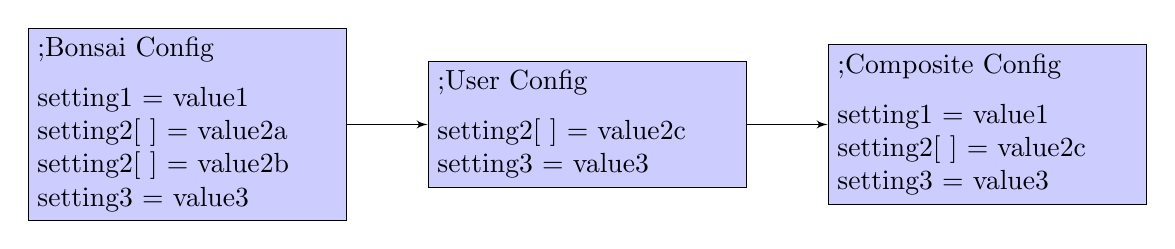
\begin{tikzpicture}
	% Place nodes
	\node [block] (bonsaiconf) {
		;Bonsai Config \\
		\vspace{6pt}
		setting1 = value1 \\
		setting2[ ] = value2a \\
		setting2[ ] = value2b \\
		setting3 = value3 \\
	};
	\node [block, right of=bonsaiconf, node distance=2in] (userconf) {
		;User Config \\
		\vspace{6pt}
		setting2[ ] = value2c \\
		setting3 = value3 \\
	};
	\node [block, right of=userconf, node distance=2in] (compconf) {
		;Composite Config \\
		\vspace{6pt}
		setting1 = value1 \\
		setting2[ ] = value2c \\
		setting3 = value3 \\
	};
	
	% Draw edges
	\path [line] (bonsaiconf) -- (userconf);
	\path [line] (userconf) -- (compconf);	    
	\end{tikzpicture}
	
	\vspace{12pt}
	
\end{figure}

Note that any arrays in your configuration will completely supersede the default config. This allows you to effectively remove values you do not want to include, but you must re-assign any values you want to keep from the default configuration when dealing with arrays.

\section{Location Constants}

Bonsai uses a handful of location constants to locate files and correctly handle relative locations. These are defined in the Bonsai.php file in the Bonsai root. By default they are defined as:

\begin{verbatim}
	    Bonsai\DOCUMENT_ROOT >> $_SERVER['DOCUMENT_ROOT']
	    Bonsai\PROJECT_ROOT  >> Location of the Bonsai.php file
	    Bonsai\SERVER_ROOT   >> Emtpy string
\end{verbatim}

These are used, respectively, to:

\begin{itemize}
	\item Locate user template and configuration files
	\item Locate bonsai template and configuration files
	\item Correctly prefix links that are stated relative to the server root
\end{itemize}

Depending on your server configuration, you may need to manually define one or more of these values before instantiating Bonsai, otherwise these values will be used for any un-defined constants when the Bonsai core initializes.

\chapter{Common Usage Examples}
\label{chapter:commonUsageExamples}

\section{Multiple Templates for One Content Entry}
\label{sec:multipleTemplates}

\section{Dynamic Node Examples}
\label{sec:dynamicNode}

\section{Vocab Examples}
\label{sec:vocabExamples}

\chapter*{Appendix}

\end{document}
